Das Wort {\em Zoooologe} bezeichnet einen im Zoo tätigen Oologen, einen
Eierkundler. 
Das Wort enthält sogar 5 Buchstaben {\texttt{o}}, wovon aber nur $4$
nebeneinander stehen.
In den folgenden Teilaufgaben geht es um Wörter, die wie das Wort
{\em Zoooologe} genau 6 Vokale und 3 Konsonanten enthalten.
\begin{teilaufgaben}
\item
Wieviele verschiedene Wörter der Länge 9 gibt es, die genau 4 benachbarte
und zwei einzelne Vokale enthalten?
\item
Wieviele verschiedene Wörter der Länge 9 gibt es, die genau
5 benachbarte Vokale und einen einzelnen Vokal enthalten?
\item 
Wieviele verschiedene Wörter der Länge 9 gibt es, die genau 6 benachbarte
Vokale enthalten?
\end{teilaufgaben}

\begin{hinweis}
Das deutsche Alphabet hat 5 Vokale und 21 Konsonanten.
\end{hinweis}

\begin{loesung}
\begin{teilaufgaben}
\item
Die Vokalgruppen können in den drei Anordnungen
\[
114, 141, 411
\]
platziert werden.
Zwischen den Vokalgruppen braucht es mindestens einen Konsonanten,
es sind aber auch zwei zulässig.
Wenn nur genau ein Konsonanten zwischen den Gruppen steht, dann gibt
es noch die Möglichkeit am Wortanfang oder Wortende einen Konsonanten zu
platzieren.
Anders ausgedrückt sind zwei Konsonanten fest vorgegeben, den dritten
kann man an vier möglichen Stellen platzieren.
Damit haben wir folgende $3\cdot 4=12$ Möglichkeiten
\[
\def\k{\texttt{k}}
\def\K{\bgroup\color{red}\texttt{k}\egroup}
\begin{matrix}
\K1\k1\k4&\K1\k4\k1&\K4\k1\k1\\
1\K\k1\k4&1\K\k4\k1&4\K\k1\k1\\
1\k1\K\k4&1\k4\K\k1&4\k1\K\k1\\
1\k1\k4\K&1\k4\k1\K&4\k1\k1\K
\end{matrix}
\]
Die sechs Vokalplätze kann man auf $5^6$ Arten belegen,
die 3 Konsonantenplätze auf $26^3$ Arten,
die Gesamtzahl der Wörter wird daher
\[
3\cdot 4 \cdot 5^6 \cdot 21^3
=
3\cdot 4 \cdot 15625 \cdot 9261
=
1736437500.
\]
\item
Es gibt gleich viele Wörter, die die 5er-Gruppe vor dem einzelnen
Vokal haben wie solche, bei denen es umgekehrt ist.
Es genügt daher, nur die eine Art Wörter zu zählen.
Ausgehend von den 3 Konsonanten gibt es vier Plätze, wo die Vokalgruppen
eingefügt werden könnten, nämlich
\[
\texttt{\textvisiblespace k\textvisiblespace k\textvisiblespace k\textvisiblespace}
\]
Zwei dieser Plätze müsse gewählt werden,
es gibt also 
$ \binom{4}{2} =6 $.
Wieder kann man die Konsonanten- und Vokalplätze auf auf
$5^6\cdot 21^3$ Arten belegen und bekommt damit
\[
2\cdot 6 \cdot5^6\cdot 21^3
=
1736437500
\]
Wörter.
Dies sind halb so viele Wörter wie in Teilaufgabe a).
\item
In diesem Fall haben wir ausgehend von den drei Konsonanten
vier Plätze, wo wir die 6 Zeichen lange Vokalgruppe platzieren können,
nämlich
\begin{center}
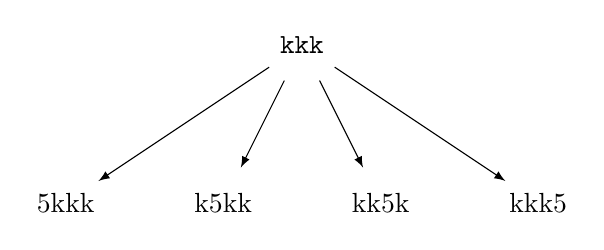
\begin{tikzpicture}[>=latex]
\node at (0,0) {\texttt{kkk}};
\draw[->,shorten >= 0.5cm,shorten <= 0.5cm] (0,0) -- (-3,-2);
\draw[->,shorten >= 0.5cm,shorten <= 0.5cm] (0,0) -- (-1,-2);
\draw[->,shorten >= 0.5cm,shorten <= 0.5cm] (0,0) -- (1,-2);
\draw[->,shorten >= 0.5cm,shorten <= 0.5cm] (0,0) -- (3,-2);
\node at (-3,-2) {\text{5kkk}};
\node at (-1,-2) {\text{k5kk}};
\node at (1,-2) {\text{kk5k}};
\node at (3,-2) {\text{kkk5}};
\end{tikzpicture}
\end{center}
Die Anzahl der Wörter ist daher
\[
4\cdot 5^6\cdot 21^3
=
578812500.
\qedhere
\]
\end{teilaufgaben}
\end{loesung}

\begin{bewertung}
Anzahl Belegungen der Konsonantenplätze $21^3$ ({\bf K}) 1 Punkt,
Anzahl Belegungen der Vokalplätze $5^6$ ({\bf V}) 1 Punkt,
In jeder Teilaufgabe: Anzahl Verteilungen der Konsonanten- und 
Vokalplätze ({\bf A}), ({\bf B}) und ({\bf C}) je 1 Punkt,
ausgerechnete Zahlenresultate ({\bf Z}) 1 Punkt.
\end{bewertung}
